%! program = pdflatex

% ajouter draft pr brouillon
% twoside
\documentclass[10pt,a4paper]{article} 

\usepackage[hmargin=2cm,vmargin=1cm]{geometry}
\renewcommand{\rmdefault}{bch} % change default font

\usepackage[english]{babel}
\usepackage[utf8]{inputenc}
\usepackage{tikz} 
\usetikzlibrary{arrows,decorations.pathmorphing,backgrounds,fit,positioning,shapes.symbols,chains}

%%%%%%%%%%%%%%%%%%%%%%%%%%%%%%%%%%%%
%%% BEGIN DOCUMENT
\begin{document}

\begin{figure}[h]

\centering
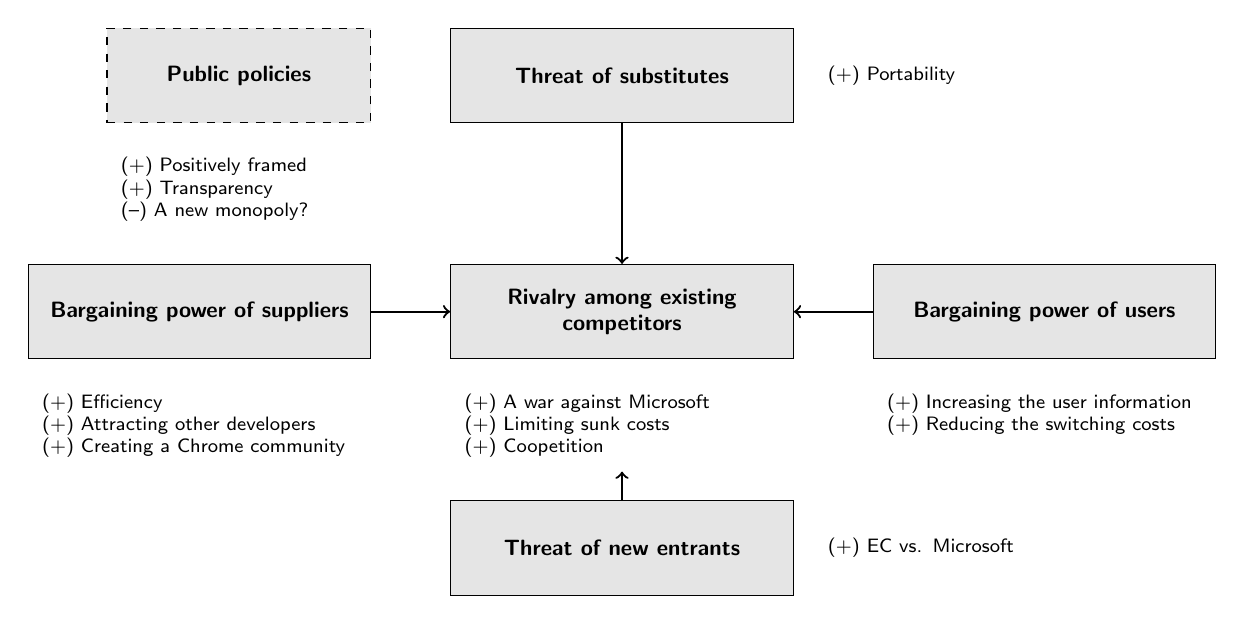
\begin{tikzpicture}
[node distance = 1cm, auto,font=\footnotesize,
% STYLES
every node/.style={node distance=3cm},
% The comment style is used to describe the characteristics of each force
comment/.style={rectangle, inner sep= 5pt, text width=4cm, node distance=0.25cm, font=\scriptsize\sffamily},
% The force style is used to draw the forces' name
force/.style={rectangle, draw, fill=black!10, inner sep=5pt, text width=4cm, text badly centered, minimum height=1.2cm, font=\bfseries\footnotesize\sffamily}] 

% Draw forces
\node [force] (rivalry) {Rivalry among existing competitors};
\node [force, above of=rivalry] (substitutes) {Threat of substitutes};
\node [force, text width=3cm, dashed, left=1cm of substitutes] (state) {Public policies};
\node [force, left=1cm of rivalry] (suppliers) {Bargaining power of suppliers};
\node [force, right=1cm of rivalry] (users) {Bargaining power of users};
\node [force, below of=rivalry] (entrants) {Threat of new entrants};

%%%%%%%%%%%%%%%
% Change data from here

% RIVALRY
\node [comment, below=0.25 of rivalry] (comment-rivalry) {(+) A war against Microsoft\\
(+) Limiting sunk costs\\
(+) Coopetition};

% SUPPLIERS
\node [comment, below=0.25cm of suppliers] {(+) Efficiency\\
(+) Attracting other developers\\
(+) Creating a Chrome community};

% SUBSTITUTES
\node [comment, right=0.25 of substitutes] {(+) Portability};

% USERS
\node [comment, below=0.25 of users] {(+) Increasing the user information\\
(+) Reducing the switching costs};

% NEW ENTRANTS
\node [comment, right=0.25 of entrants] {(+) EC vs. Microsoft};

% PUBLIC POLICIES
\node [comment, text width=3cm, below=0.25 of state] {(+) Positively framed\\
(+) Transparency\\
(--) A new monopoly?};

%%%%%%%%%%%%%%%%

% Draw the links between forces
\path[->,thick] 
(substitutes) edge (rivalry)
(suppliers) edge (rivalry)
(users) edge (rivalry)
(entrants) edge (comment-rivalry);

\end{tikzpicture} 
\caption{FOSS in Chrome influences industry structure by increasing competition}
\label{fig:6forces}
\end{figure}

\end{document}